\documentclass[11pt,aspectratio=169]{beamer}

\usetheme{Madrid}
\usecolortheme{seahorse}

\usepackage[utf8]{inputenc}
\usepackage{amsmath,amssymb}
\usepackage{algpseudocode}
\usepackage{algorithmicx}
\usepackage{xcolor}
\usepackage{listings}
\usepackage{booktabs}
\usepackage{tikz}
\usetikzlibrary{arrows.meta,positioning,fit,backgrounds}

\setbeamertemplate{navigation symbols}{}
\setbeamertemplate{footline}[frame number]

\lstdefinestyle{py}{
  language=Python,
  basicstyle=\ttfamily\scriptsize,
  keywordstyle=\color{blue!70!black}\bfseries,
  commentstyle=\color{gray},
  stringstyle=\color{green!40!black},
  showstringspaces=false,
  breaklines=true,
  numbers=left,
  numberstyle=\tiny\color{gray},
  frame=single,
  xleftmargin=1.5em,
  aboveskip=0.3em,
  belowskip=0.3em
}

\title{LeetCode Deep Dive}
\subtitle{From First Instinct to Optimal Algorithm: Game DP and State-Space BFS in
Practice\\
\small Week 13 Supplement -- TOAE209/TOAH209: Design and Analysis of Algorithms}
\author{Foreign Trade University}
\date{}

\begin{document}

% ---------------------------------------------------------------
\begin{frame}
  \titlepage
\end{frame}
% ---------------------------------------------------------------

\begin{frame}{Outline}
  \tableofcontents
\end{frame}

% =================================================================
\section{A Framework for Attacking a New Search/Game Problem}
% =================================================================

\begin{frame}{Why walk through LeetCode problems?}
  \begin{itemize}
    \item This week's \texttt{LEETCODE.md} list gives you eight Week 13 problems to
    \emph{practice on your own}. This deck instead \textbf{narrates the thinking
    process} for two of them, end to end, so you can reuse the process on the rest.
    \item We pick one \textcolor{blue!50!black}{\textbf{Medium}} (\emph{Stone Game}) and
    one \textcolor{red!60!black}{\textbf{Hard}} (\emph{Word Ladder}) -- one is a
    two-player \textbf{game} solved by memoized minimax-style DP, the other is a huge
    implicit \textbf{state space} tamed by BFS with pruning.
    \item Both are exactly this week's two big ideas in miniature: a game whose
    exponential-looking tree collapses to a polynomial number of \emph{distinct}
    states, and a search space too large to enumerate, made tractable by exploring it
    breadth-first with a visited set instead of blindly.
  \end{itemize}
\end{frame}

\begin{frame}{The four-step process we will repeat twice}
  \begin{enumerate}
    \item \textbf{First instinct.} Write down the algorithm that follows most directly
    from re-reading the problem statement -- usually ``simulate every choice both
    players could make'' or ``search every path.''
    \item \textbf{Measure why it hurts.} Compute the actual complexity, plug in the
    problem's constraints, and see the number blow up.
    \item \textbf{Find the structural insight.} Ask: \emph{how many genuinely distinct
    states are there, really?} Almost always far fewer than the number of \emph{paths}
    to reach them.
    \item \textbf{Implement the optimal algorithm}, trace it by hand on a small example,
    then look for the \emph{programming-level} (not algorithmic) tricks that make the
    implementation itself correct and fast.
  \end{enumerate}
  \begin{alertblock}{This mirrors the course}
    Steps 1--3 are this week's ``exponential tree $\to$ polynomially many \emph{states}''
    story (minimax $\to$ memoized game DP, bounded search trees); step 4 turns a correct
    algorithm into working code.
  \end{alertblock}
\end{frame}

% =================================================================
\section{Problem 1 (Medium): Stone Game}
% =================================================================

\begin{frame}{Problem statement}
  \begin{block}{LeetCode 877 -- Stone Game (\textcolor{blue!50!black}{Medium})}
    An \textbf{even} number of piles of stones are arranged in a row; pile $i$ has
    \texttt{piles[i]} stones (the total is odd, so no ties are possible). Alex and Lee
    alternate turns, Alex first; each turn, a player removes the entire pile from
    \textbf{either end} of the remaining row and adds its stones to their own score.
    Both play \textbf{optimally} to maximize their own final score. Return
    \texttt{true} if Alex wins.
  \end{block}
  \begin{itemize}
    \item Constraints (LeetCode): $2 \le \texttt{piles.length} \le 500$ (even),
    $1 \le \texttt{piles[i]} \le 500$.
    \item This is exactly this week's \textbf{minimax} game tree: at each node, the
    player to move picks the child (take-left or take-right) that is best \emph{for
    them}, and the two players alternate the max/min role.
  \end{itemize}
\end{frame}

\begin{frame}{Worked example}
  \begin{columns}
  \begin{column}{0.5\textwidth}
  \texttt{piles = [5, 3, 4, 5]}
  \begin{center}
  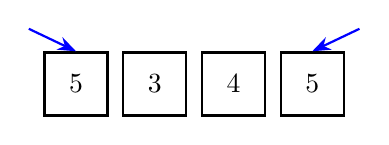
\begin{tikzpicture}[
      pile/.style={draw, thick, minimum width=8mm, minimum height=8mm},
      >=Stealth]
    \foreach \i/\v/\x in {0/5/0,1/3/1,2/4/2,3/5/3}
      \node[pile] (p\i) at (\x,0) {\v};
    \draw[->, thick, blue] (-0.6,0.7) -- (p0.north);
    \draw[->, thick, blue] (3.6,0.7) -- (p3.north);
  \end{tikzpicture}
  \\[2pt]
  {\scriptsize each turn: take the leftmost or rightmost remaining pile}
  \end{center}
  \end{column}
  \begin{column}{0.5\textwidth}
  \small
  \begin{itemize}
    \item Alex moves first, then Lee, alternating, until all $4$ piles are gone.
    \item Both play optimally for \emph{themselves} -- Alex is not trying to minimize
    Lee's score, only to maximize his own (the classic subtlety of general-sum-looking
    but actually zero-sum-difference games).
    \item \textbf{Answer:} \texttt{true} -- with \emph{both} playing optimally, Alex
    wins $9$ stones to Lee's $8$ (we derive this score exactly, not by guessing, on the
    trace slide below).
  \end{itemize}
  \end{column}
  \end{columns}
\end{frame}

\begin{frame}{First instinct: simulate the whole game tree}
  \begin{block}{Most direct reading of the problem}
    ``Both play optimally'' $\Rightarrow$ recursively try both choices (take-left,
    take-right) for whoever's turn it is, and let each player pick whichever leads to
    the better outcome \emph{for them}.
  \end{block}
  \begin{algorithmic}[1]
    \Function{Play}{piles, turn}
      \If{piles is empty} \Return $(0, 0)$ \Comment{(Alex total, Lee total)} \EndIf
      \State $\textit{left} \gets \Call{Play}{\text{piles without first pile}, \lnot
      turn}$ \Comment{add first pile to \textit{turn}'s side}
      \State $\textit{right} \gets \Call{Play}{\text{piles without last pile}, \lnot
      turn}$ \Comment{add last pile to \textit{turn}'s side}
      \State \Return whichever of \textit{left}, \textit{right} gives \textit{turn} the
      larger score
    \EndFunction
  \end{algorithmic}
\end{frame}

\begin{frame}{Why this is bad}
  \begin{itemize}
    \item Each call branches into $2$ recursive calls (take-left or take-right), and
    the recursion is $n$ turns deep $\Rightarrow O(2^n)$ leaves.
    \item Plug in the constraint: $n = 500 \Rightarrow 2^{500} \approx 3\times 10^{150}$
    -- vastly more than the number of atoms in the observable universe ($\sim 10^{80}$).
    This is not ``slow,'' it is \textbf{uncomputable} in the lifetime of the universe.
  \end{itemize}
  \begin{alertblock}{The smell to notice}
    The recursion tree has $2^n$ \emph{leaves}, but look at what each call actually
    depends on: only \emph{which contiguous slice of piles remains}. Many different
    take-left/take-right \emph{sequences} land on the exact same remaining slice --
    that repetition is the wasted work.
  \end{alertblock}
\end{frame}

\begin{frame}{The structural insight}
  \begin{itemize}
    \item After any sequence of moves, the remaining piles are always a
    \textbf{contiguous window} $\texttt{piles}[i..j]$ -- there are only
    $\binom{n+1}{2} = O(n^2)$ such windows, versus $2^n$ move sequences.
    \item Reformulate with a \textbf{score-difference} trick: let $dp[i][j]$ be the
    largest possible \emph{(current player's score $-$ opponent's score)} achievable by
    whoever moves first on window $[i,j]$. Then
    \[
      dp[i][j] = \max\big(\texttt{piles}[i] - dp[i{+}1][j],\ \ \texttt{piles}[j] -
      dp[i][j{-}1]\big),
    \]
    with base case $dp[i][i] = \texttt{piles}[i]$.
    \item Alex wins iff $dp[0][n-1] > 0$ -- because $dp[0][n-1]$ is exactly
    (Alex's total) $-$ (Lee's total) under optimal play by both.
  \end{itemize}
\end{frame}

\begin{frame}{Optimal algorithm: pseudocode}
  \footnotesize
  \begin{algorithmic}[1]
    \Function{StoneGame}{piles}
      \State $n \gets \texttt{len(piles)}$
      \State $dp[i][i] \gets \texttt{piles}[i]$ for all $i$ \Comment{windows of length 1}
      \For{$\textit{len} \gets 2$ \textbf{to} $n$} \Comment{grow the window size}
        \For{$i \gets 0$ \textbf{to} $n - \textit{len}$}
          \State $j \gets i + \textit{len} - 1$
          \State $dp[i][j] \gets \max(\texttt{piles}[i] - dp[i{+}1][j],\ \texttt{piles}[j]
          - dp[i][j{-}1])$
        \EndFor
      \EndFor
      \State \Return $dp[0][n-1] > 0$
    \EndFunction
  \end{algorithmic}
  $O(n^2)$ time, $O(n^2)$ space -- versus the $O(2^n)$ naive tree.
\end{frame}

\begin{frame}{Trace on the worked example}
  \scriptsize
  \texttt{piles = [5, 3, 4, 5]}; fill $dp[i][j]$ by increasing window length.
  \begin{center}
  \begin{tabular}{@{}c c c c@{}}
    \toprule
    window & length 1 & length 2 & length 3 / 4 \\
    \midrule
    $[0,0],[1,1],[2,2],[3,3]$ & $5,\ 3,\ 4,\ 5$ & & \\
    $[0,1]$ & & $\max(5{-}3,\,3{-}5)=2$ & \\
    $[1,2]$ & & $\max(3{-}4,\,4{-}3)=1$ & \\
    $[2,3]$ & & $\max(4{-}5,\,5{-}4)=1$ & \\
    $[0,2]$ & & & $\max(5{-}dp[1,2]{=}1,\ 4{-}dp[0,1]{=}2)=\max(4,2)=4$ \\
    $[1,3]$ & & & $\max(3{-}dp[2,3]{=}1,\ 5{-}dp[1,2]{=}1)=\max(2,4)=4$ \\
    $[0,3]$ & & & $\max(5{-}dp[1,3]{=}4,\ 5{-}dp[0,2]{=}4)=\max(1,1)=1$ \\
    \bottomrule
  \end{tabular}
  \end{center}
  $dp[0][3] = 1 > 0 \Rightarrow$ \textbf{true} -- matches LeetCode's expected output.
  Unwinding \emph{which} choice achieved each max gives one concrete optimal line: Alex
  takes pile $0$ ($5$), Lee takes pile $3$ ($5$), Alex takes pile $2$ ($4$), Lee takes
  pile $1$ ($3$) -- Alex $9$, Lee $8$, difference $1$, totalling $17$. \checkmark
\end{frame}

\begin{frame}{Complexity: naive vs.\ optimal}
  \begin{center}
  \begin{tabular}{@{}lll@{}}
    \toprule
    Approach & Time & At $n=500$ \\
    \midrule
    Full game tree (naive) & $O(2^n)$ & $\approx 3\times 10^{150}$ \\
    \textbf{Interval DP (score difference)} & $\boldsymbol{O(n^2)}$ & $250{,}000$ \\
    \bottomrule
  \end{tabular}
  \end{center}
  The naive recursion is not merely slower -- it visits $2^{500}$ tree nodes to answer
  a question that only has $\binom{501}{2}\approx 125{,}250$ \emph{distinct} states.
  Recognizing ``how many distinct states, really?'' is the entire gap.
\end{frame}

\begin{frame}[fragile]{Python implementation}
  \begin{lstlisting}[style=py]
def stoneGame(piles):
    n = len(piles)
    dp = [[0] * n for _ in range(n)]
    for i in range(n):
        dp[i][i] = piles[i]                # window of length 1

    for length in range(2, n + 1):         # grow the window
        for i in range(n - length + 1):
            j = i + length - 1
            dp[i][j] = max(piles[i] - dp[i + 1][j],
                            piles[j] - dp[i][j - 1])

    return dp[0][n - 1] > 0
  \end{lstlisting}
  \vspace{0.3em}
  \small Filling by increasing \texttt{length} guarantees $dp[i{+}1][j]$ and
  $dp[i][j{-}1]$ (both \emph{shorter} windows) are already computed before $dp[i][j]$
  needs them.
\end{frame}

\begin{frame}{Implementation tips \& tricks (the programming side)}
  \small
  \begin{itemize}
    \item \textbf{Fill order is not optional.} The recurrence needs shorter windows
    computed first; a loop nested the ``obvious'' way (outer $i$, inner $j$) accidentally
    reads $dp[i][j-1]$ or $dp[i+1][j]$ \emph{before} it has been written. Looping by
    \texttt{length} (as above) sidesteps the bug entirely instead of reasoning about
    loop-order edge cases.
    \item \textbf{\texttt{@lru\_cache} recursion vs.\ the bottom-up array.} A memoized
    recursive version is easier to write correctly first (translate the recurrence
    almost verbatim) but pays Python function-call overhead per state and needs
    \texttt{sys.setrecursionlimit} raised for $n=500$; the bottom-up array above has
    neither cost and is the version to submit.
    \item \textbf{Space can drop to $O(n)$.} Each diagonal only reads the
    \emph{previous} diagonal's values, so a single rolling 1-D array (updated carefully
    in decreasing $i$ order within each \texttt{length} pass) suffices -- a standard
    interval-DP space optimization once the $O(n^2)$ version is verified correct.
  \end{itemize}
\end{frame}

% =================================================================
\section{Problem 2 (Hard): Word Ladder}
% =================================================================

\begin{frame}{Problem statement}
  \begin{block}{LeetCode 127 -- Word Ladder (\textcolor{red!60!black}{Hard})}
    Given \texttt{beginWord}, \texttt{endWord}, and a dictionary \texttt{wordList},
    return the number of words in the \textbf{shortest} transformation sequence from
    \texttt{beginWord} to \texttt{endWord}, where each step changes exactly \textbf{one
    letter} and every intermediate word must appear in \texttt{wordList}. Return $0$ if
    no such sequence exists.
  \end{block}
  \begin{itemize}
    \item Constraints (LeetCode): $1 \le \texttt{wordList.length} \le 5000$, all words
    the same length $L \le 10$.
    \item Reframe it as a graph problem: nodes are words, an edge joins two words that
    differ in exactly one letter, and the answer is a \textbf{shortest path} in this
    (huge, implicit) graph -- exactly this week's ``exponential-looking search space,
    tamed by exploring it the right way'' theme.
  \end{itemize}
\end{frame}

\begin{frame}{Worked example}
  \small
  \texttt{beginWord = "hit"}, \texttt{endWord = "cog"}\\
  \texttt{wordList = ["hot","dot","dog","lot","log","cog"]}
  \begin{center}
  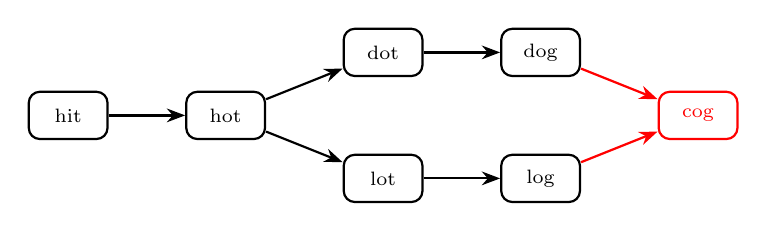
\begin{tikzpicture}[
      w/.style={draw, thick, rounded corners, minimum width=10mm, minimum height=6mm,
      font=\scriptsize},
      >=Stealth]
    \node[w] (hit) at (0,0) {hit};
    \node[w] (hot) at (2,0) {hot};
    \node[w] (dot) at (4,0.8) {dot};
    \node[w] (lot) at (4,-0.8) {lot};
    \node[w] (dog) at (6,0.8) {dog};
    \node[w] (log) at (6,-0.8) {log};
    \node[w,red] (cog) at (8,0) {cog};
    \draw[->,thick] (hit)--(hot);
    \draw[->,thick] (hot)--(dot);
    \draw[->,thick] (hot)--(lot);
    \draw[->,thick] (dot)--(dog);
    \draw[->,thick] (lot)--(log);
    \draw[->,thick,red] (dog)--(cog);
    \draw[->,thick,red] (log)--(cog);
  \end{tikzpicture}
  \end{center}
  Two equally-short paths exist: \texttt{hit-hot-dot-dog-cog} and
  \texttt{hit-hot-lot-log-cog}, both length $5$. \textbf{Answer:} $5$.
\end{frame}

\begin{frame}{First instinct: search every path}
  \begin{block}{Most direct reading of the problem}
    ``Find the shortest transformation sequence'' $\Rightarrow$ DFS/backtrack from
    \texttt{beginWord}, trying every one-letter change at each step, exploring every
    path to \texttt{endWord}, and keep the shortest one found.
  \end{block}
  \begin{algorithmic}[1]
    \Function{DFS}{word, path}
      \If{word $=$ endWord} record \texttt{len(path)}; \Return \EndIf
      \For{each 1-letter variant $v$ of word in wordList}
        \State \Call{DFS}{$v$, path $+ [v]$} \Comment{no record of what's already
        been tried!}
      \EndFor
    \EndFunction
  \end{algorithmic}
\end{frame}

\begin{frame}{Why this is bad}
  \begin{itemize}
    \item Without tracking visited words, the search can loop between words forever
    (\texttt{hot} $\to$ \texttt{dot} $\to$ \texttt{hot} $\to \cdots$) -- it may not even
    \textbf{terminate}.
    \item Even with a visited check per path (not globally), DFS must explore
    \emph{every} path before it can be sure it found the \emph{shortest} one -- in a
    graph with up to $5000$ words and roughly $25L\!\approx\!250$ possible one-letter
    edits per word, the number of distinct paths explodes combinatorially long before
    reaching \texttt{endWord}.
  \end{itemize}
  \begin{alertblock}{The smell to notice}
    ``Explore every path to find the \emph{shortest} one'' is always the wrong move in
    an unweighted graph -- \textbf{BFS} finds shortest paths by construction, without
    ever exploring a path longer than necessary.
  \end{alertblock}
\end{frame}

\begin{frame}{Structural insight \#1: this is unweighted shortest path}
  \begin{itemize}
    \item Every edge (one-letter change) has the same ``cost'' -- so the shortest
    transformation sequence is exactly the \textbf{BFS shortest path} from
    \texttt{beginWord} to \texttt{endWord}, layer by layer, with a \textbf{global
    visited set} so no word is ever processed twice.
    \item This bounds the work to (number of words) $\times$ (edits per word) instead of
    (number of \emph{paths}) -- BFS visits each of the $\le 5000$ words \textbf{at most
    once}.
  \end{itemize}
\end{frame}

\begin{frame}{Structural insight \#2: how you \emph{find} neighbors matters too}
  \begin{itemize}
    \item \textbf{Tier 1 (correct, but not optimal):} precompute the graph by comparing
    \emph{every pair} of words for a one-letter difference: $O(N^2 L)$ -- at
    $N{=}5000,\,L{=}10$, that is $2.5\times10^8$ character comparisons.
    \item \textbf{Tier 2 (optimal):} from each word, \emph{generate} its $\le 25L$
    one-letter variants directly and test dictionary membership in $O(1)$ via a hash
    set -- $O(NL \cdot 26)$ total, about $1.3\times10^6$ operations at the same
    constraints, roughly $190\times$ fewer.
    \item The lesson: even after picking the right \emph{algorithm} (BFS), \emph{how}
    you enumerate a node's neighbors can itself be an asymptotic improvement.
  \end{itemize}
\end{frame}

\begin{frame}{BFS trace on the worked example}
  \scriptsize
  Visited set starts as \texttt{\{hit\}}; \texttt{wordSet =
  \{hot,dot,dog,lot,log,cog\}}.
  \begin{center}
  \begin{tabular}{@{}c p{2.4cm} p{7.4cm}@{}}
    \toprule
    layer (length) & frontier & how it was reached \\
    \midrule
    $1$ & \texttt{hit} & start \\
    $2$ & \texttt{hot} & \texttt{hit}$\to$\texttt{hot} (1 letter); \texttt{dot, lot,
    log, dog, cog} each differ from \texttt{hit} by $\ge 2$ letters -- not neighbors \\
    $3$ & \texttt{dot, lot} & both differ from \texttt{hot} by exactly $1$ letter;
    \texttt{log, dog, cog} do not \\
    $4$ & \texttt{dog, log} & \texttt{dog} from \texttt{dot}; \texttt{log} from
    \texttt{lot} (each $1$ letter) \\
    $5$ & \texttt{cog} & \texttt{cog} reachable from \emph{both} \texttt{dog} and
    \texttt{log} -- first one processed wins, length is the same either way \\
    \bottomrule
  \end{tabular}
  \end{center}
  \texttt{cog} first appears at layer $5$ $\Rightarrow$ \textbf{answer: 5} -- matches
  the expected output.
\end{frame}

\begin{frame}{Optimal algorithm: pseudocode}
  \footnotesize
  \begin{algorithmic}[1]
    \Function{WordLadder}{beginWord, endWord, wordList}
      \State $\textit{words} \gets$ set(wordList) \Comment{$O(1)$ membership}
      \If{endWord $\notin$ words} \Return $0$ \EndIf
      \State queue $\gets [(\text{beginWord}, 1)]$; remove beginWord from \textit{words}
      \While{queue not empty}
        \State $(word, dist) \gets$ queue.popleft()
        \If{word $=$ endWord} \Return $dist$ \EndIf
        \For{each position $p$ in word, each letter $c \neq word[p]$}
          \State $v \gets$ word with position $p$ replaced by $c$
          \If{$v \in \textit{words}$}
            \State remove $v$ from \textit{words}; enqueue $(v, dist+1)$
          \EndIf
        \EndFor
      \EndWhile
      \State \Return $0$
    \EndFunction
  \end{algorithmic}
  \scriptsize $O(NL\cdot26)$ total -- each of the $\le N$ words is enqueued once.
\end{frame}

\begin{frame}{Complexity: naive vs.\ optimal}
  \begin{center}
  \begin{tabular}{@{}lll@{}}
    \toprule
    Approach & Time & At $N=5000,\,L=10$ \\
    \midrule
    DFS, explore every path & exponential & does not finish \\
    BFS over precomputed all-pairs graph & $O(N^2 L)$ & $\approx 2.5\times10^8$ \\
    \textbf{BFS, generate variants on the fly} & $\boldsymbol{O(NL\cdot26)}$ &
    $\approx 1.3\times10^6$ \\
    \bottomrule
  \end{tabular}
  \end{center}
  Two separate wins stack: BFS over DFS (bounds work by \emph{states}, not
  \emph{paths}), and generate-neighbors over compare-all-pairs (bounds work by
  \emph{edits}, not \emph{other words}).
\end{frame}

\begin{frame}[fragile]{Python implementation (part 1: setup)}
  \begin{lstlisting}[style=py]
from collections import deque
import string

def ladderLength(beginWord, endWord, wordList):
    words = set(wordList)
    if endWord not in words:
        return 0

    queue = deque([(beginWord, 1)])
    words.discard(beginWord)     # double duty: dictionary AND visited set
  \end{lstlisting}
\end{frame}

\begin{frame}[fragile]{Python implementation (part 2: BFS loop)}
  \begin{lstlisting}[style=py]
    while queue:
        word, dist = queue.popleft()
        if word == endWord:
            return dist
        for i in range(len(word)):
            prefix, suffix = word[:i], word[i + 1:]
            for c in string.ascii_lowercase:
                if c == word[i]:
                    continue
                candidate = prefix + c + suffix
                if candidate in words:
                    words.discard(candidate)   # mark visited before enqueueing
                    queue.append((candidate, dist + 1))

    return 0
  \end{lstlisting}
\end{frame}

\begin{frame}{Implementation tips \& tricks (the programming side)}
  \small
  \begin{itemize}
    \item \textbf{\texttt{deque.popleft()}, never \texttt{list.pop(0)}.} Popping the
    front of a Python \texttt{list} is $O(n)$ (it shifts every remaining element);
    \texttt{collections.deque} makes it $O(1)$. Using a plain list here would silently
    turn an $O(NL\cdot26)$ algorithm back into something quadratic in the queue size.
    \item \textbf{Reuse the dictionary set as the visited set.} Calling
    \texttt{words.discard(candidate)} the moment a word is \emph{enqueued} (not when it
    is \emph{processed}) means membership testing and visited-tracking are the same
    $O(1)$ hash-set operation -- no second data structure needed, and no risk of the
    same word being enqueued twice from two different parents in the same layer.
    \item \textbf{Build each candidate with slicing, not a mutable list.}
    \texttt{prefix + c + suffix} on Python strings is a small, cheap allocation; a
    tempting alternative (convert to \texttt{list(word)}, mutate one index, \texttt{"".join(...)}) does strictly more work for the same result.
    \item \textbf{Bonus (borderline algorithmic):} \emph{bidirectional} BFS -- growing
    frontiers from \texttt{beginWord} and \texttt{endWord} simultaneously, always
    expanding whichever frontier is smaller -- is the standard further speed-up for
    this exact problem, cutting the effective branching from $b^d$ to roughly
    $2b^{d/2}$.
  \end{itemize}
\end{frame}

% =================================================================
\section{Summary}
% =================================================================

\begin{frame}{Summary: two problems, one lesson}
  \footnotesize
  \begin{enumerate}
    \item \textbf{Stone Game} has an exponential-looking game tree ($2^n$ move
    sequences), but only $O(n^2)$ \emph{genuinely distinct} states (contiguous
    windows) -- memoized interval DP collapses the tree onto those states.
    \item \textbf{Word Ladder} has an exponential-looking search space (every path
    through an implicit word graph), but BFS bounds the work by the number of
    \emph{states} (words) rather than the number of \emph{paths} between them --
    and generating neighbors on the fly (instead of precomputing all pairs) shaves a
    further factor of $N/26L$ off that.
    \item Both times, the naive instinct was ``enumerate everything that could
    happen''; both times, the fix was to notice that \emph{most of what could happen
    revisits the same underlying state}, and to compute each state's answer exactly
    once -- the same move as this week's bounded search trees and memoized game DP.
    \item The implementation tricks (fill order, \texttt{deque} vs.\ \texttt{list},
    reusing one set for two jobs) are a second, independent layer: even the
    \emph{optimal} algorithm can regress to a worse complexity class through an
    innocent-looking data-structure choice.
  \end{enumerate}
  \begin{alertblock}{Keep practicing}
    \texttt{LEETCODE.md} lists six more Week 13 problems (\emph{Sliding Puzzle},
    \emph{Smallest Sufficient Team}, \emph{Can I Win}, \emph{Cat and Mouse}, \dots) --
    try applying the same four-step process to each of them.
  \end{alertblock}
\end{frame}

\end{document}
